\section{Introduction and Architecture}

\subsection{Purpose and Design}
Monitoring Unix server environments is critical for preventing resource exhaustion, diagnosing performance degradation, and maintaining service availability. However, system observability on Unix platforms presents unique engineering challenges. Traditional command-line tools like \texttt{top}, \texttt{vmstat}, and \texttt{iostat} provide instantaneous status but lack historical aggregation, automated anomaly detection, and intuitive visualizations. Conversely, enterprise observability suites  impose substantial resource footprints, complex daemon dependencies, and intrusive probe effects on host systems, often altering the very performance characteristics they intend to measure.

The goal of our project is to deliver an autonomous, zero-configuration Unix monitoring and alerting suite engineered strictly for minimal probe overhead. The system operates end-to-end without external databases, third-party agents, or mandatory network services, using deterministic, filesystem-backed CSV and JSON contracts.

The end-to-end pipeline consists of four distinct operational stages:
\begin{enumerate}
    \item \textbf{Data Collection:} A lightweight,  Bash background daemon (\texttt{bin/collector.sh}) samples 16 core system metrics directly from Linux \texttt{/proc} and \texttt{/sys} pseudofiles at 5-second intervals and records the top-5 resource-consuming processes.
    \item \textbf{Data Cleaning:} A pure-Python engine (\texttt{src/cleaner.py}) validates metric bounds, deduplicates timestamps, forward-fills brief transient gaps ($\le 15$~s), and tags statistical outliers using Median Absolute Deviation (MAD) without discarding historical records.
    \item \textbf{Statistical Analysis:} An analytics engine (\texttt{src/analyzer.py}) computes rolling window statistics (1h, 24h, 7d, all), and normalizes process utilization across CPU cores. End to end system integration and testing.
    \item \textbf{Alerting and Serving:} A rule evaluator (\texttt{src/alerts.py}) tracks sustained threshold conditions and cooldowns, while a local Flask server (\texttt{src/server.py}) and responsive dashboard (\texttt{web/}) deliver real-time streaming activity dials and historical trends.
\end{enumerate}

\begin{figure}[htbp]
    \centering
    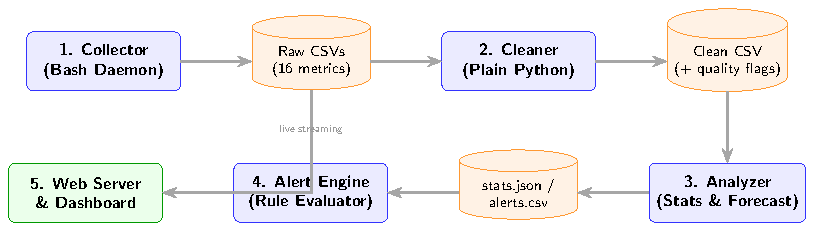
\includegraphics[width=0.92\textwidth]{figures/pipeline_arch.pdf}
    \caption{SysMon End-to-End System Architecture and Data Pipeline}
    \label{fig:pipeline_arch}
\end{figure}

The project development was divided into distinct subsystem responsibilities among five team members:
\begin{itemize}
    \item \textbf{Integrator + Analysis (Varun J Kumar):} Repository initialization, master launcher (\texttt{./sysmon}), pipeline orchestrator (\texttt{bin/run\_pipeline.sh}), statistical analysis engine (\texttt{src/analyzer.py}), multi-core profiling, and documentation. End to end system integration and testing.
    \item \textbf{Collector + Cleaner (Sri Harsha Rangu):} Bash metric daemon (\texttt{bin/collector.sh}), daemon lifecycle scripts, and data cleaning engine (\texttt{src/cleaner.py}).
    \item \textbf{Frontend (Prerit Devashetti):} HTML5/CSS web dashboard, real-time Chart.js streaming visualizer, radial gauge dials, and multi-page UI views.
    \item \textbf{Backend / Server (Amogh Chhuneja):} Flask REST API endpoints, real-time streaming metric merge, and server test suites.
    \item \textbf{Alerts + Synthetic Data + Profiling (Amitha Reddy Kota and Amulya Koti):} Threshold alert engine (\texttt{src/alerts.py}), synthetic data generator (\texttt{bin/gen\_data.py}), and stress test harness (\texttt{bin/stress.sh}).
\end{itemize}

\subsection{Inputs and Outputs}
Table~\ref{tab:metrics_columns} enumerates all 16 raw system metrics captured by the collector into \texttt{data/raw/metrics\_YYYYMMDD.csv}.

\begin{table}[htbp]
    \centering
    \small
    \begin{tabular}{rlll}
        \toprule
        \# & Column & Description & Kernel / Command Source \\
        \midrule
        1 & \texttt{epoch} & Unix timestamp in seconds & \texttt{date +\%s} \\
        2 & \texttt{iso\_time} & UTC timestamp (ISO 8601) & \texttt{date -u +"\%Y-\%m-\%dT\%H:\%M:\%SZ"} \\
        3 & \texttt{cpu\_pct} & Overall CPU utilization (\%) & Delta calculation from \texttt{/proc/stat} \\
        4 & \texttt{mem\_used\_pct} & RAM utilization (\%) & Calculated from \texttt{/proc/meminfo} \\
        5 & \texttt{mem\_avail\_mb} & Available physical memory (MB) & \texttt{MemAvailable} in \texttt{/proc/meminfo} \\
        6 & \texttt{swap\_used\_pct} & Swap utilization (\%) & \texttt{SwapTotal}, \texttt{SwapFree} in \texttt{/proc/meminfo} \\
        7 & \texttt{disk\_used\_pct} & Root partition utilization (\%) & \texttt{df -P /} \\
        8 & \texttt{load1} & 1-minute system load average & First field of \texttt{/proc/loadavg} \\
        9 & \texttt{load5} & 5-minute system load average & Second field of \texttt{/proc/loadavg} \\
        10 & \texttt{load15} & 15-minute system load average & Third field of \texttt{/proc/loadavg} \\
        11 & \texttt{net\_rx\_kbps} & Network receive speed (kB/s) & Delta from \texttt{/proc/net/dev} \\
        12 & \texttt{net\_tx\_kbps} & Network transmit speed (kB/s) & Delta from \texttt{/proc/net/dev} \\
        13 & \texttt{cpu\_temp\_c} & Package CPU temperature ($^\circ$C) & \texttt{/sys/class/thermal/thermal\_zone*} \\
        14 & \texttt{gpu\_util\_pct} & GPU core load (\%) & \texttt{nvidia-smi} or AMD sysfs \\
        15 & \texttt{gpu\_mem\_used\_pct} & GPU VRAM utilization (\%) & \texttt{nvidia-smi} or AMD sysfs \\
        16 & \texttt{gpu\_temp\_c} & GPU temperature ($^\circ$C) & \texttt{nvidia-smi} or AMD sysfs \\
        \bottomrule
    \end{tabular}
    \caption{All 16 Raw Telemetry Metrics Captured in the Metrics CSV}
    \label{tab:metrics_columns}
\end{table}

\subsection{Testing and Results}
The end-to-end architecture was validated using automated test suites across all 5 tiers. Table~\ref{tab:intro_test} summarizes the verification scope and results.

\begin{table}[htbp]
    \centering
    \small
    \begin{tabular}{lll}
        \toprule
        Subsystem & Verification Scope & Outcome \\
        \midrule
        Collector Daemon & 16-column schema compliance, PID locking, stop trap & Passed (100\% clean samples) \\
        Data Cleaner & Deduplication, gap forward-filling, MAD outlier flags & Passed (Zero dropped valid rows) \\
        Statistical Analyzer & Rolling windows (1h, 24h, 7d, all), OLS disk forecast & Passed (Validated against fixtures) \\
        Alert Engine & Sustained rule breaches ($N=3$), cooldown timers & Passed (Zero alert storms) \\
        Web Server \& UI & REST endpoints, streaming Chart.js graph, process table & Passed ($<20$~ms local response) \\
        \bottomrule
    \end{tabular}
    \caption{Subsystem End-to-End Validation Summary}
    \label{tab:intro_test}
\end{table}

\subsection{Limitations}
Flat-file CSV storage does not scale efficiently to multi-month historical archives without noticeable query latency during linear scans. Metric sampling is interval-driven via a 5-second timer rather than interrupt-driven via kernel eBPF tracepoints.
